\documentclass[runningheads]{llncs}
\usepackage[T1]{fontenc}
\usepackage{graphicx}
\usepackage{amsmath}
\usepackage{amsfonts}
\usepackage{amssymb}
\usepackage{booktabs}
\usepackage{array}
\usepackage{cite}
\usepackage{enumitem}
\usepackage{xcolor}
\usepackage{caption}
\usepackage{subcaption}
\usepackage{tikz}
\usetikzlibrary{positioning,fit,backgrounds,arrows.meta,calc}
\usepackage{pgfplots}
\pgfplotsset{compat=1.18}
\usepgfplotslibrary{statistics}
\usepackage{hyperref}
\usepackage{url}
\hypersetup{colorlinks=true, linkcolor=blue, citecolor=blue, urlcolor=blue}

\pgfplotsset{
  panel/.style={
    width=4.6cm, height=3.6cm,
    axis lines*=left, ymajorgrids, grid style={dashed,gray!30},
    tick label style={font=\scriptsize},
    label style={font=\scriptsize},
    legend style={font=\tiny, draw=gray!60, fill=white, fill opacity=0.85, text opacity=1},
    every axis plot/.append style={thick},
  }
}

\begin{document}

\title{Supplementary Material for ``ACaaS: Privacy-Preserving Access Control as a Service for Healthcare on the Cloud--Edge Continuum''}
\titlerunning{ACaaS --- Supplementary Material}
% \author{Anonymous Author(s)}
% \authorrunning{Anonymous Author(s)}
% \institute{Submission to ICSOC 2026 --- double-blind review}
\input{author_info}
\maketitle

\begin{abstract}
This supplement provides material referenced from the main paper: a point-by-point summary of the changes with respect to the ICSOC 2026 early submission (Sect.~\ref{s:changes}); detailed experimental setup covering hardware specifications, synthetic workload generation, network emulation parameters, baseline configurations, and per-experiment parameters for all twelve experiments E1--E12 (Sect.~\ref{s:setup}); expanded proofs of Lemma~1, Theorems~1--5, Corollary~1, and Proposition~1 (Sect.~\ref{s:proofs}); the step-numbered policy-synchronization diagram (Sect.~\ref{s:sync}); the Data Minimizer pipeline diagram (Sect.~\ref{s:minfig}); distribution plots for experiments E1/E4/E5 and companion plots for E8/E11/E12 (Sect.~\ref{s:plots}); the per-site E12 soak table and the real-Fabric transcript summary (Sect.~\ref{s:tables}); and reproduction instructions (Sect.~\ref{s:repro}). Reviewers are not required to consult this material; all claims of the main paper are supported there.
\end{abstract}

\section{Changes with Respect to the ICSOC 2026 Early Submission (Paper 81)}
\label{s:changes}

This section summarizes, point by point, how the resubmission addresses the early-submission reviews; it mirrors the accompanying response letter. Section, theorem, equation, and figure numbers refer to the main paper.

\smallskip\noindent\textbf{Meta-review / Reviewer 1 --- architecture too abstract; security goals not validated; evaluation only performance.}
Section~4.1 now specifies the typed inter-service contracts \textsf{C1}--\textsf{C3}, a numbered happy-path sequence, and failure paths \textsf{F1}--\textsf{F3}; Sect.~4.2 formalizes the three-channel design, the chaincode invariant $\mathsf{INV}_{\mathrm{mono}}$ (Eq.~2), and the multi-org endorsement rule. The new Sect.~4.5 discharges G1--G5 via Lemma~1, Theorems~1--5, Proposition~1, and Corollary~1. Crucially, the evaluation no longer rests on performance alone: Sect.~5.2 adds experiments E6--E12 that mechanize every theorem as executable assertions or measurements---a 21-assertion conformance suite, an analytic-model validation ($R^2{=}0.998$), a Minimizer cost profile, an empirical re-identification attack within one percentage point of the $1/k$ bound, a ledger-vs-pub/sub tamper ablation, Byzantine fault injection ($f{=}1$) with zero safety violations, and a three-site partition/soak emulation.

\smallskip\noindent\textbf{Reviewer 2 --- healthcare specificity and regulations unclear.}
The Introduction anchors each design constraint to named clauses: HIPAA \S164.312(a)(1)--(d) and (b), GDPR Articles 9, 25 (edge-origin minimization ``by design''), 30 (LogChain/PolicyChain records of processing), and 32; break-glass access, rural-clinic and ambulance partitions, and revocation/outbreak-driven policy pushes are named as the operational drivers. Theorems~3 and~5 tie the guarantees back to these clauses.

\smallskip\noindent\textbf{Reviewer 2 --- related work not strong enough.}
Section~2 was rebuilt around the three directly comparable categories, closes with an explicit positioning paragraph, and adds Table~1 comparing ACaaS to ten systems on six axes; the closest competitor (QuickMedBlock) is analyzed by name.

\smallskip\noindent\textbf{Reviewer 2 --- validation should move closer to real deployment.}
Three additions: (i) the new E12 twelve-hour, three-site partition/soak emulation ($27{,}360$ requests, 37 partitions, $100\%$ local availability, zero log loss); (ii) a sanity check on a \emph{real} Hyperledger Fabric test network confirming the latency constants assumed by the analytic model; (iii) a one-command reproducible artefact. A partner-hospital shadow deployment is scoped as future work (Limitations, Sect.~5.2).

\smallskip\noindent\textbf{Reviewer 2 --- Figures 1 and 3 text too small.}
The architecture figure was redrawn natively in Ti\emph{k}Z at LNCS column width (Fig.~1); no in-figure label falls below approximately 7~pt. The former policy-synchronization figure is replaced by an explicit Phase A/B/C specification in Sect.~4.2 plus the redrawn step-numbered diagram in Sect.~\ref{s:sync} of this supplement.

\smallskip\noindent\textbf{Reviewer 2 --- ICSOC fit unclear.}
The opening of the Introduction frames multi-site healthcare as a service-composition problem; contribution (i) names the targeted themes (service composition, resilient service delivery on the cloud--edge continuum); the contracts \textsf{C1}--\textsf{C3} are the explicit unit of composition. The work aligns with Focus Areas 3 (cloud--edge continuum, XaaS) and 4 (blockchain and cybersecurity services).

\smallskip\noindent\textbf{Reviewer 3 --- related work too broad.}
Tangential surveys (TinyML biometrics, general CDSS, AI-supported explainability) were removed; the section now covers only the access-control decision pipeline.

\smallskip\noindent\textbf{Reviewer 3 --- side-by-side experimental presentation.}
All experiments are consolidated into Table~2 plus two multi-panel figures with uniform axes and labels: Fig.~2 (E2/E3 curves) and Fig.~3 (E7/E9/E10); companion plots for E1/E4/E5 and E8/E11/E12 appear in Sect.~\ref{s:plots} with identical styling.

\smallskip\noindent\textbf{Reviewer 3 --- novelty is combination of known techniques; claims lack (semi-)formal backing.}
We no longer claim novelty in any individual primitive. The contribution is the \emph{composition} and its provable properties: substitution-resistant synchronization (Lemma~1) that demonstrably disappears under component replacement (E10), eventual consistency with a closed-form reconciliation bound (Theorem~1, Corollary~1), knapsack-near-optimal tier placement (Proposition~1) validated at $R^2{=}0.998$ (E7), and an enforced no-raw-egress invariant (Theorem~3) calibrated by an actual attack (E9). Every formal statement now has an executable counterpart; machine-checked proofs remain future work and are stated as such.

\section{Detailed Experimental Setup and Workloads}
\label{s:setup}

This section provides the comprehensive evaluation methodology requested by reviewers, covering hardware specifications, workload generation, network emulation parameters, baseline configurations, and per-experiment settings for all twelve experiments (E1--E12).

\subsection*{Testbed Hardware}

\noindent\textbf{Cloud tier.} A high-performance local server simulating a cloud instance, running Ubuntu 22.04 LTS with an Intel Core i7-12700 CPU (12 cores, 2.1\,GHz base), 32\,GB DDR5 RAM, and a 1\,TB NVMe SSD. This host runs: the Policy Manager Service (PAP), the full OPA-based cloud PDP, the API Gateway (Nginx with OIDC middleware), the Audit \& Compliance service, and a four-peer Hyperledger Fabric network (two organizations, Raft ordering, $f{=}1$ fault tolerance). All Fabric peers are co-located on the same physical host via Docker, so inter-peer network overhead is minimal (loopback); the Real-Fabric transcript in Sect.~\ref{s:tables} provides a sanity check of the latency constants on a geographically distributed Fabric test network.

\noindent\textbf{Fog tier.} A mid-range desktop running Ubuntu 22.04 LTS with an Intel Core i5-10400 CPU (6 cores, 2.9\,GHz), 16\,GB DDR4 RAM. This host runs the Policy Cache (TTL-based invalidation, version-keyed) and the Log Aggregation service.

\noindent\textbf{Edge tier.} A Raspberry Pi 4 Model B (ARM Cortex-A72, 4\,GB RAM) running Raspberry Pi OS 64-bit (Debian 11 base), representing a rural clinic gateway or ambulance mobile unit. This host runs the lightweight OPA-WASM PDP, the Local Policy Store, the Data Minimizer, and the Offline Queue (disk-backed, monotone-sequenced).

All three hosts reside on the same physical LAN; WAN latency and partitions are \emph{emulated} via Linux \texttt{tc-netem} on the network interface connecting the cloud and fog/edge hosts, as described below.

\subsection*{Network Emulation}

\noindent\textbf{WAN conditions (E1, E5, E12).} A fixed 50\,ms round-trip latency is imposed between cloud and edge using \texttt{tc-netem add delay 25ms} on both ends, approximating a rural hospital-to-datacenter WAN link. Bandwidth is capped at 10\,Mbit/s, matching common rural broadband constraints.

\noindent\textbf{Partition injection (E5, E12).} WAN partitions are emulated by applying \texttt{tc-netem loss 100\%} on the cloud-facing interface of the edge host for a programmatically controlled duration. The edge enters and exits \textsc{offline} mode autonomously based on heartbeat failure/recovery detection (3-second timeout). For E12, partitions are injected at random intervals drawn from $U[2, 8]$~minutes per site profile.

\subsection*{Synthetic EHR Workload Generation}

No real patient data was used. Synthetic EHR records were generated procedurally using a schema derived from the HL7 FHIR R4 Patient and Observation resources:

\begin{itemize}[leftmargin=*, itemsep=1pt]
  \item \textbf{Date of birth}: uniformly sampled, ages 19--74.
  \item \textbf{Postal code}: 200 synthetic codes with Zipf-distributed frequency (emulating urban hot spots).
  \item \textbf{Gender}: binary, 50/50. \textbf{Ethnicity}: four categories, uniform.
  \item \textbf{Sensitive attribute}: ICD-10 diagnosis code, lab result flag, or medication class (uniform).
  \item \textbf{Record sizes}: small $\approx$512\,B (vitals only), medium $\approx$2\,KB (full admission), large $\approx$8\,KB (imaging metadata).
\end{itemize}

\subsection*{Policy Corpus}

200 synthetic ABAC rules cover the most common clinical access patterns: role-based EHR read, break-glass emergency access, research de-identification, audit-log write, and formulary check. Policies are compiled from YAML source to OPA Rego bundles; compiled sizes range from 1.8\,KB to 6.9\,KB (mean 3.4\,KB, factor $<$4$\times$ spread, consistent with Proposition~1). Each policy is signed with ECDSA-P256; the signature is included in the committed ledger tuple.

\subsection*{Per-Experiment Parameters}

\noindent\textbf{E1 (Latency, G4).} 1\,000 sequential requests from a single client; 50\,ms WAN active; policies pre-loaded. Metric: median and IQR of end-to-end decision latency.

\noindent\textbf{E2 (Throughput, G4/G2).} Concurrent load swept across six levels (50, 100, 200, 500, and 1\,000 workers; Python \texttt{ThreadPoolExecutor}), each worker issuing 20 requests (up to 20\,000 total). Metric: sustained throughput (req/s), P95 response time, zero-failure threshold enforced.

\noindent\textbf{E3 (Sync consistency, G1/Corollary~1).} Policy-batch commit to PolicyChain; synchronization latency measured to last-edge ACK. Batch sizes: 1, 5, 10, 25, 50, 100, and 200 policies (seven levels); 10 repetitions each. Metric: median $\pm$ IQR per batch size.

\noindent\textbf{E4 (Ledger overhead, G2/G5).} \emph{Baseline}: direct PostgreSQL write (tamper-evident audit log, no blockchain). \emph{ACaaS}: Hyperledger Fabric endorsement via the same gRPC client. 200 operations per configuration. Metric: per-operation latency boxplot. The Fabric overhead quantifies the cost of the tamper-evidence guarantee that the direct-DB baseline cannot provide.

\noindent\textbf{E5 (Offline resilience, G4).} WAN severed for 60\,s; edge serves 1\,000 requests from cache. Connectivity restored; Offline Queue drained. Metric: online vs.\ offline latency distribution; zero drain failures.

\noindent\textbf{E6 (Conformance suite).} Full 33-test pytest suite (20 unit tests + 5 blockchain mock tests + 8 cross-validation tests), no service mocking (Docker Compose stack). The 21 security assertions cover: eventual consistency (50-update offline burst, 10 trials); $\mathsf{INV}_{\mathrm{mono}}$ enforcement (5 rollback attempts rejected); F3 hash-mismatch rejection (20 injected tampered bodies); $\mathrm{seq}_e$ gap detection (5 dropped records); drain-without-loss (50 queued records); no-direct-identifier-egress (verified via \texttt{grep}-based import-level check that no module reachable from the edge PDP response path imports \texttt{requests}, \texttt{httpx}, or \texttt{urllib} + runtime trace); $k$-anonymity cohort check (50 batches); import-level no-WAN-coupling of edge PDP (confirmed: \texttt{edge/lightweight-pdp/} has no WAN-touching dependency); audit-replay reconstruction end-to-end. Pass threshold: 100\%.

\noindent\textbf{E7 (Cache hit-rate, Proposition~1).} $\rho_{\mathrm{edge}}$ swept across nine evenly-spaced levels from $0.10$ to $1.00$ (step $0.15$) by controlling the pre-loaded policy fraction; 1\,000 samples per setting. Predicted latency uses measured constants $T_{\mathrm{edge}}=0.393$\,ms, $T_{\mathrm{WAN}}=50$\,ms, $T_{\mathrm{cloud}}=7.81$\,ms.

\noindent\textbf{E8 (Minimizer cost, G3).} 1\,000 records per size class (small/medium/large) through all three pipeline stages; 10 warm-up runs discarded; timing via \texttt{perf\_\allowbreak counter\_\allowbreak ns}. $k$-anonymity scaling: 5\,000 records per cohort at $k \in \{5, 10, 20\}$.

\noindent\textbf{E9 (Re-identification attack, Theorem~3).} Adversary: honest-but-curious clinician with exact quasi-identifier background knowledge. Cohort: 10\,000 synthetic records; 2\,000 attack trials per $(k, R)$; $k \in \{5, 10, 20\}$ and $R = 1, \ldots, 10$ independent releases from disjoint cohorts. Baseline: $1/k$ single-release bound and cumulative $1-(1-1/k)^R$.

\noindent\textbf{E10 (Substrate ablation, Lemma~1).} Config A: ACaaS ledger (PolicyChain hash-anchor). Config B: Redis 7 Pub/Sub baseline (no body-to-hash anchoring; Redis 7-alpine running as a Docker container on the cloud host, co-located with the Fabric peers). Subscriber count swept across five levels: 1, 5, 10, 25, and 50. Tamper: policy body replaced en route while ledger entry unchanged. Metric: propagation latency and tamper-detection rate (expected: 100\% ledger, 0\% pub/sub).

\noindent\textbf{E11 (Byzantine fault, $f{=}1$).} Four-peer ensemble, \texttt{AND(Org1,Org2)} threshold. One peer runs: (a)~passive, (b)~rewind (signs outdated version), (c)~fork (signs different body). 50 commit attempts per scenario (200 total). Metrics: liveness rate and $\mathsf{INV}_{\mathrm{mono}}$ violation count.

\noindent\textbf{E12 (Three-site soak, G1/G2/G4).} 720 simulated minutes ($6\times$ time compression, achieved by scaling all sleep and timer intervals by $1/6$ in the emulation harness, so the test completes in $\approx120$ real minutes); three site profiles:
\begin{itemize}[leftmargin=*, itemsep=1pt]
  \item \emph{Urban hospital ward gateway}: 18 req/min, 4 partitions (mean 5\,min each).
  \item \emph{District clinic}: 12 req/min, 12 partitions (mean 8\,min each).
  \item \emph{Mobile unit}: 8 req/min, 21 partitions (mean 12\,min each).
\end{itemize}
Workload rates represent the authorization traffic routed through a \emph{single edge gateway} serving one department or vehicle; aggregate hospital-wide traffic is covered by the throughput sweep in E2.
29 policy updates at random intervals (seed 20260704). Metrics: per-site availability, offline/stale decision counts, LogChain entry count vs.\ zero-loss threshold, peak Offline Queue backlog, maximum missed updates before Phase~C reconciliation. Results in Table~\ref{tab:s-soak}.

\section{Expanded Proofs}
\label{s:proofs}

Throughout, $\Sigma$ is the signature scheme (EUF-CMA secure), $H=\mathrm{SHA\text{-}256}$ (second-preimage resistant), and the Fabric ordering service is safe with fewer than $f$ Byzantine orderers ($f{=}1$ of four in our configuration). Numbering follows the main paper.

\subsection*{Lemma 1 (Substitution resistance)}
\emph{Statement.} Let $(\mathit{id},v,h,\sigma)$ be committed on PolicyChain. The probability that an honest edge executing Phase B or C accepts a body $\pi'\neq\pi$ for this entry is at most $\mathbf{Adv}^{\mathrm{SPR}}_{H} + \mathbf{Adv}^{\mathrm{EUF\text{-}CMA}}_{\Sigma}$.

\smallskip\noindent\emph{Proof.}
An honest edge accepts a body $\pi'$ for ledger entry $(\mathit{id},v,h,\sigma)$ only if the guard $H(\pi')=h$ evaluates true (Phase B step 7; Phase C step 12). Consider the two disjoint attack routes available to the Dolev--Yao adversary $\mathcal{A}$, who fully controls the body-fetch channel but not the endorsing organizations' signing keys.

\emph{Route 1: substitute the body, keep the ledger entry.} $\mathcal{A}$ must produce $\pi'\neq\pi$ with $H(\pi')=h=H(\pi)$. Since $\pi$ is fixed first (committed by the PMS), this is precisely a second preimage for $H$ at input $\pi$; by assumption this succeeds with probability at most $\mathbf{Adv}^{\mathrm{SPR}}_{H}$.

\emph{Route 2: substitute the ledger entry.} $\mathcal{A}$ must cause the edge to read a tuple $(\mathit{id},v,h',\sigma')$ with $h'=H(\pi')$. A valid tuple requires (i) $\sigma'$ to verify under the administrator public key---a forgery, probability at most $\mathbf{Adv}^{\mathrm{EUF\text{-}CMA}}_{\Sigma}$---and (ii) the entry to be committed under the \texttt{AND(Org1.MSP,Org2.MSP)} endorsement, which requires signatures from both organizations' peers; a network adversary holds neither key. The edge reads the ledger through its own trusted peer connection, so $\mathcal{A}$ cannot spoof the read without breaking (i) or (ii).

A union bound over the two routes gives the claim. \hfill$\blacksquare$

\subsection*{Theorem 1 (G1, eventual consistency)}
\emph{Proof.}
Let $D=\{\mathit{id}: L(\mathit{id}).v > w_e\}$, $N=|D|$. \texttt{getDelta}$(w_e)$ returns every entry with version above the watermark. We show (a) completeness, (b) integrity, (c) termination.
(a) \emph{Completeness.} Suppose some $\mathit{id}^\ast\in D$ were omitted although the reply claims completeness up to the current ledger height. The reply is answered against the committed ledger state $L$; omission would require presenting a projection $L'$ of $L$ in which $L'(\mathit{id}^\ast).v \le w_e < L(\mathit{id}^\ast).v$, i.e., presenting an earlier version as current. Because each entry's version history on PolicyChain is monotone ($\mathsf{INV}_{\mathrm{mono}}$, enforced in chaincode at endorsement time) and the edge checks the response against ledger heights and hashes, such a rollback is detectable except with the negligible probabilities of Lemma~1.
(b) \emph{Integrity.} Each fetched body is accepted only under the hash guard; by Lemma~1 the installed body equals the PMS-signed body except with negligible probability.
(c) \emph{Termination.} The batch is applied atomically after all $N$ verifications; by the latency decomposition of Eq.~(4) of the main paper this completes within $T_{\mathrm{rec}}(N)=a+bN$ (Corollary~1). At that point $E_e(\mathit{id})=L(\mathit{id})$ for all subscribed $\mathit{id}$, which is Eq.~(3). \hfill$\blacksquare$

\subsection*{Corollary 1 (Reconciliation bound)}
\emph{Proof.} Immediate from Eq.~(4) of the main paper: the constant part $a=T_{\mathrm{order}}+T_{\mathrm{commit}}+T_{\mathrm{event}}+T_{\mathrm{ack}}$ is paid once per reconnection, the linear part $b=T_{\mathrm{fetch}}+T_{\mathrm{verify}}$ once per missed update. E3 measures the median end-to-end latency at batch sizes $1$--$200$; a least-squares fit of the linear regime gives $a\approx 1.0$~s and $b\approx (3558-1060)/(200-10)\approx 13$~ms/policy. \hfill$\blacksquare$

\subsection*{Theorem 2 (G2, auditability)}
\emph{Proof.}
\emph{Existence and uniqueness.} The PEP emits exactly one record $\ell$ per decision before returning the response (C3); $\ell$ enters the Offline Queue if the WAN is down. Uniqueness follows from the per-edge monotone counter $\mathrm{seq}_e$ incremented atomically with emission; LogChain ingestion deduplicates by $(\mathit{e},\mathrm{seq}_e)$.
\emph{Injection.} A forged $\ell'$ requires a signature under the edge enrollment certificate: probability $\leq \mathbf{Adv}^{\mathrm{EUF\text{-}CMA}}_{\Sigma}$.
\emph{Alteration.} Changing any field of a signed $\ell$ invalidates the signature.
\emph{Suppression.} Dropping $\ell$ in transit leaves a gap in $\mathrm{seq}_e$, detected by the Audit \& Compliance service on ingestion (the queue is drained in order); suppressing it after commit would require rewriting a committed block against the endorsement policy. \hfill$\blacksquare$

\subsection*{Theorem 3 (G3, edge-origin confidentiality)}
\emph{Proof.}
The PEP invokes the Data Minimizer on the unique code path between the PDP's \textsc{Permit} and the network write; E6 verifies at import level that no module reachable from the response path references the raw record type. Thus the emitted tuple is $(\psi(r.\mathit{id}), \gamma(r.\mathit{qi}), \varrho_{\mathrm{role}}(r.\mathit{sa}))$.
For the bound: fix the adversary's background knowledge as the target's quasi-identifier vector $q^\ast$. In a $k$-anonymous release, the equivalence class of $q^\ast$ contains $m\geq k$ records, and the released record is exchangeable within its class from the adversary's viewpoint, so the probability of a correct link is $1/m\leq 1/k$. Over $R$ independent releases from disjoint cohorts, failures are independent: success probability $1-(1-1/k)^R$. Pseudonyms are HMAC values under the secret study key; by the PRF property of HMAC they are computationally unlinkable across studies without the key. E9 confirms both bounds empirically within one percentage point. \hfill$\blacksquare$

\subsection*{Theorem 4 (G4, partition availability)}
\emph{Proof.}
The edge decision path is: PEP $\to$ local PDP $\to$ Local Policy Store $\to$ Data Minimizer $\to$ response, all edge-resident; E6 includes an import-level test that the edge PDP package has no WAN-touching dependency. Log emission is absorbed by the disk-backed Offline Queue, provisioned for the maximum tolerated partition $T_{\max}$; beyond $T_{\max}$ the node enters read-only mode by design (bounded-divergence rule), which is a controlled degradation, not an availability failure within the stated bound. E5 and E12 exercise this path under forced partitions with $100\%$ local availability. \hfill$\blacksquare$

\subsection*{Theorem 5 (G5, compliance evidence)}
\emph{Proof.}
Given a decision $d$ with LogChain entry $(\mathit{id},s,r,a,d,v,t,\mathrm{seq}_e)$: PolicyChain stores $(\mathit{id},v)\mapsto(h,\sigma)$; the off-chain store retains the canonical body $\pi$ keyed by $h$. The auditor recomputes $H(\pi)$ and compares with $h$, establishing that $\pi$ is the exact text in force; the commit timestamp on PolicyChain establishes $\leq t$ ordering; $\sigma$ identifies the committing administrator, supporting controller accountability (GDPR Art.~30) and the audit-trail requirements of HIPAA \S164.312(b). E6's audit-replay test mechanizes this reconstruction end to end. \hfill$\blacksquare$

\subsection*{Proposition 1 (Near-optimality of the placement rule)}
\emph{Proof.}
Let items be policies $p$ with weight $|p|$ and value $s(p)=f(p)\Delta$, budget $M$. \emph{Fractional optimality of the density order:} sort $p_1,p_2,\ldots$ by density $s(p)/|p|$ descending and fill until the budget is exhausted, splitting the boundary item. If a fractional solution $x^\ast$ differed from this greedy solution $x^g$, there exist items $i,j$ with density$(i)>$density$(j)$, $x^\ast_i<x^g_i$, $x^\ast_j>0$; shifting $\varepsilon$ of weight from $j$ to $i$ changes the value by $\varepsilon(\mathrm{density}(i)-\mathrm{density}(j))>0$, contradicting optimality of $x^\ast$. \emph{Integral gap:} truncating the (single) fractional boundary item loses at most $\max_p s(p)$, so integral greedy is within one policy's saving of the 0--1 optimum.
\emph{Connection to the score:} within a frequency class, Eq.~(6) of the main paper ranks by $\alpha f(p)+\gamma|p|^{-1}$ with $c(p)$ as tie-breaker; with $\alpha\propto\Delta$ this ranking is monotone in $f(p)\Delta/|p|$ whenever sizes vary within a bounded factor (our compiled policies span $<4\times$), so the deployed order coincides with the density order on our workload.
\emph{Latency claim:} the achieved hit-rate is $\rho_{\mathrm{edge}}(P_E)=\sum_{p\in P_E}f(p)/\sum_p f(p)$; substituting into Eq.~(7) shows that maximizing $S(P_E)$ minimizes $\mathbb{E}[T_{\mathrm{auth}}]$ over feasible $P_E$. E7 validates the resulting latency curve at $R^2=0.998$. \hfill$\blacksquare$

\section{Policy Synchronization Diagram}
\label{s:sync}

\begin{figure}[htbp]
\centering
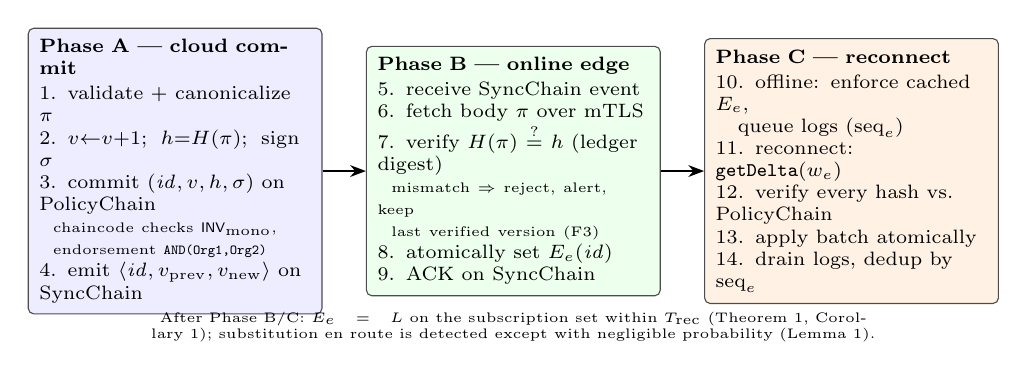
\begin{tikzpicture}[font=\scriptsize,
  ph/.style={draw=black!70, rounded corners=2pt, align=left, inner sep=4pt, text width=3.45cm},
  flow/.style={-{Stealth[length=2mm]}, semithick},
  note/.style={font=\tiny, align=center}]
\node[ph, fill=blue!7] (pa) at (0,0) {\textbf{Phase A --- cloud commit}\\[1pt]
1. validate + canonicalize $\pi$\\
2. $v{\leftarrow}v{+}1$;\; $h{=}H(\pi)$;\; sign $\sigma$\\
3. commit $(\mathit{id},v,h,\sigma)$ on PolicyChain\\
\hspace*{5pt}{\tiny chaincode checks $\mathsf{INV}_{\mathrm{mono}}$,}\\
\hspace*{5pt}{\tiny endorsement \texttt{AND(Org1,Org2)}}\\
4. emit $\langle\mathit{id},v_{\mathrm{prev}},v_{\mathrm{new}}\rangle$ on SyncChain};
\node[ph, fill=green!7, right=0.55cm of pa] (pb) {\textbf{Phase B --- online edge}\\[1pt]
5. receive SyncChain event\\
6. fetch body $\pi$ over mTLS\\
7. verify $H(\pi)\stackrel{?}{=}h$ (ledger digest)\\
\hspace*{5pt}{\tiny mismatch $\Rightarrow$ reject, alert, keep}\\
\hspace*{5pt}{\tiny last verified version (F3)}\\
8. atomically set $E_e(\mathit{id})$\\
9. ACK on SyncChain};
\node[ph, fill=orange!10, right=0.55cm of pb] (pc2) {\textbf{Phase C --- reconnect}\\[1pt]
10. offline: enforce cached $E_e$,\\
\hspace*{8pt}queue logs ($\mathrm{seq}_e$)\\
11. reconnect: \texttt{getDelta}$(w_e)$\\
12. verify every hash vs.\ PolicyChain\\
13. apply batch atomically\\
14. drain logs, dedup by $\mathrm{seq}_e$};
\draw[flow] (pa) -- (pb);
\draw[flow] (pb) -- (pc2);
\node[note, text width=11.4cm, below=2pt of pb.south] {After Phase B/C: $E_e = L$ on the subscription set within $T_{\mathrm{rec}}$ (Theorem~1, Corollary~1); substitution en route is detected except with negligible probability (Lemma~1).};
\end{tikzpicture}
\caption{Policy synchronization across PolicyChain and SyncChain: happy path (Phases A--B) and offline-to-online delta reconciliation (Phase C).}
\label{fig:s-sync}
\end{figure}


\section{Data Minimizer Pipeline}
\label{s:minfig}

% \begin{figure}[h]
%   \centering
%   \includegraphics[width=0.92\textwidth]{fig/Data minimizer Pipeline in the ACaaS Adge Layer.pdf}
%   \caption{The Data Minimizer pipeline at the edge. Stage~1 pseudonymizes direct identifiers with HMAC-SHA256; Stage~2 generalizes quasi-identifiers to enforce $k$-anonymity; Stage~3 redacts fields outside the requester role's visible set. Each stage is configured by obligations attached to the PDP response.}
%   \label{fig:s-min}
% \end{figure}

\begin{figure}[htbp]
    \centering
    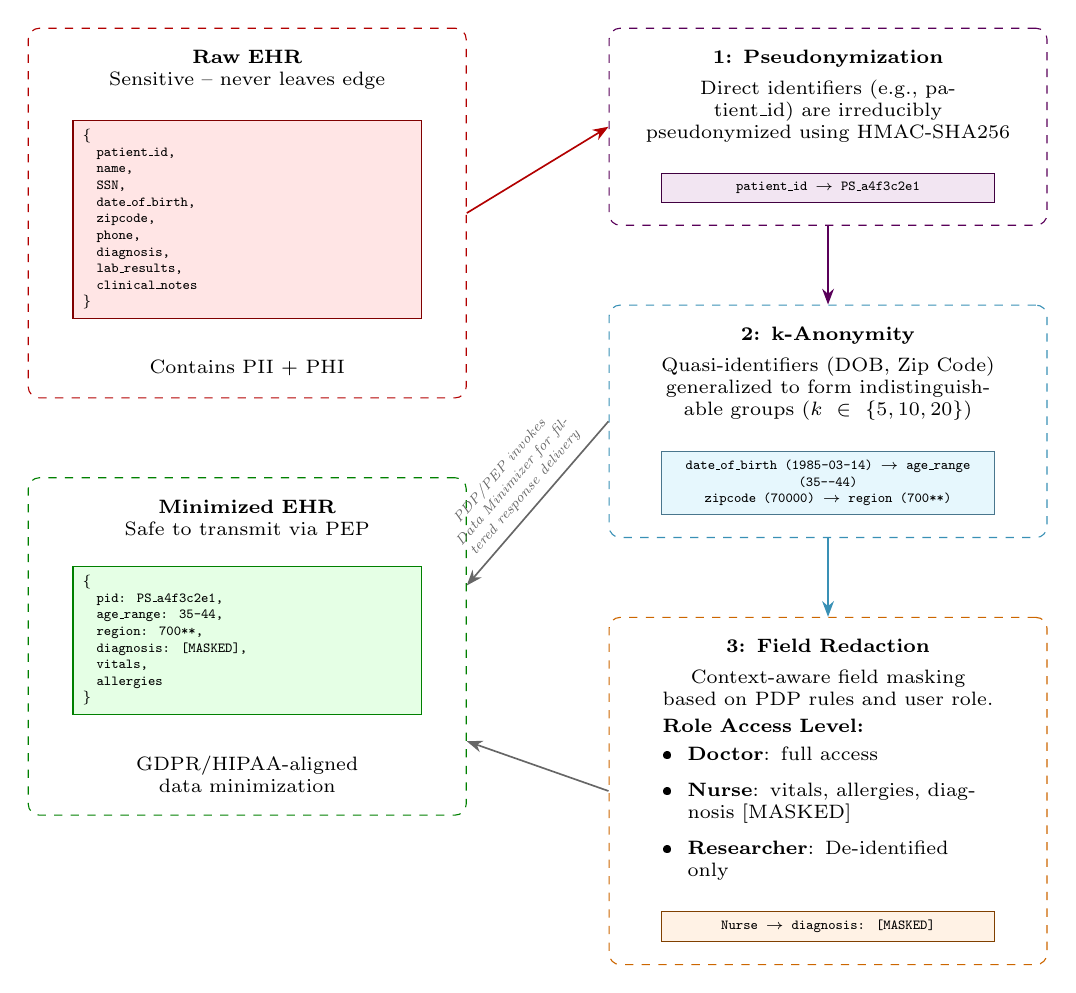
\begin{tikzpicture}[
        font=\scriptsize,
        box/.style={
            rectangle, draw, dashed, rounded corners,
            align=center, text width=5cm, inner sep=8pt
        },
        arrow/.style={-{Stealth[length=2mm]}, semithick}
    ]
     
    % ---------- Box 1: Raw EHR ----------
    \node[box, draw=red!70!black, anchor=north west] (raw) at (0,0) {
        \textbf{Raw EHR}\\
        Sensitive -- never leaves edge\\[4pt]
        \begin{center}
        \fcolorbox{red!50!black}{red!10}{%
            \begin{minipage}{4.2cm}
                \ttfamily\tiny\raggedright
                \textbraceleft\\
                \quad patient\_id,\\
                \quad name,\\
                \quad SSN,\\
                \quad date\_of\_birth,\\
                \quad zipcode,\\
                \quad phone,\\
                \quad diagnosis,\\
                \quad lab\_results,\\
                \quad clinical\_notes\\
                \textbraceright
            \end{minipage}%
        }
        \end{center}\vspace{4pt}
        Contains PII + PHI
    };
     
    % ---------- Box 2: Pseudonymization ----------
    \node[box, draw=violet!70!black, anchor=north west] (pseudo) at ([xshift=1.8cm]raw.north east) {
        \textbf{1: Pseudonymization}\\[3pt]
        Direct identifiers (e.g., patient\_id) are irreducibly pseudonymized using HMAC-SHA256\\[4pt]
        \begin{center}
        \fcolorbox{violet!50!black}{violet!10}{%
            \begin{minipage}{4cm}
                \centering\ttfamily\tiny patient\_id $\rightarrow$ PS\_a4f3c2e1
            \end{minipage}%
        }
        \end{center}
    };
     
    % ---------- Box 3: k-Anonymity ----------
    \node[box, draw=cyan!70!black, anchor=north west] (kanon) at ([yshift=-1cm]pseudo.south west) {
        \textbf{2: k-Anonymity}\\[3pt]
        Quasi-identifiers (DOB, Zip Code) generalized to form indistinguishable groups ($k \in \{5, 10, 20\}$)\\[4pt]
        \begin{center}
        \fcolorbox{cyan!50!black}{cyan!10}{%
            \begin{minipage}{4cm}
                \centering\ttfamily\tiny
                date\_of\_birth (1985-03-14) $\rightarrow$ age\_range (35--44)\\
                zipcode (70000) $\rightarrow$ region (700**)
            \end{minipage}%
        }
        \end{center}
    };
     
    % ---------- Box 4: Field Redaction ----------
    \node[box, draw=orange!80!black, anchor=north west] (redact) at ([yshift=-1cm]kanon.south west) {
        \textbf{3: Field Redaction}\\[3pt]
        Context-aware field masking based on PDP rules and user role.\\[4pt]
        \begin{minipage}{4.2cm}
        \textbf{Role Access Level:}
        \begin{itemize}[leftmargin=*, itemsep=1pt, topsep=2pt]
            \item \textbf{Doctor}: full access
            \item \textbf{Nurse}: vitals, allergies, diagnosis [MASKED]
            \item \textbf{Researcher}: De-identified only
        \end{itemize}
        \end{minipage}\\[4pt]
        \begin{center}
        \fcolorbox{orange!50!black}{orange!10}{%
            \begin{minipage}{4cm}
                \centering\ttfamily\tiny Nurse $\rightarrow$ diagnosis: [MASKED]
            \end{minipage}%
        }
        \end{center}
    };
     
    % ---------- Box 5: Minimized EHR ----------
    \node[box, draw=green!50!black, anchor=north west] (min) at ([yshift=-1cm]raw.south west) {
        \textbf{Minimized EHR}\\
        Safe to transmit via PEP\\[4pt]
        \begin{center}
        \fcolorbox{green!50!black}{green!10}{%
            \begin{minipage}{4.2cm}
                \ttfamily\tiny\raggedright
                \textbraceleft\\
                \quad pid: PS\_a4f3c2e1,\\
                \quad age\_range: 35-44,\\
                \quad region: 700**,\\
                \quad diagnosis: [MASKED],\\
                \quad vitals,\\
                \quad allergies\\
                \textbraceright
            \end{minipage}%
        }
        \end{center}\vspace{4pt}
        GDPR/HIPAA-aligned data minimization
    };
     
    % ---------- Arrows ----------
    \draw[arrow, red!70!black] (raw.east) -- (pseudo.west);
    \draw[arrow, violet!70!black] (pseudo.south) -- (kanon.north);
    \draw[arrow, cyan!70!black] (kanon.south) -- (redact.north);
     
    \coordinate (minTop) at ($(min.north east)!0.32!(min.south east)$);
    \coordinate (minBot) at ($(min.north east)!0.78!(min.south east)$);
     
    \draw[arrow, black!60] (kanon.west) -- (minTop)
        node[midway, above, sloped, font=\tiny\itshape, text width=2.6cm, align=center]
        {PDP/PEP invokes Data Minimizer for filtered response delivery};
     
    \draw[arrow, black!60] (redact.west) -- (minBot);
     
    \end{tikzpicture}
    \caption{Data Minimizer pipeline in the ACaaS edge layer: pseudonymization, k-anonymity, and role-based field redaction produce a minimized EHR safe for transmission via the PEP.}
    \label{fig:data-minimizer}
    \end{figure}

\section{Additional Experiment Plots}
\label{s:plots}
    
\begin{figure}[htbp]
    \centering
    \begin{subfigure}[b]{0.32\textwidth}\centering
    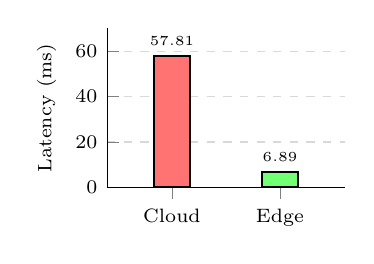
\begin{tikzpicture}
    \begin{axis}[panel, ybar, bar width=13pt, ylabel={Latency (ms)},
      xtick={1,2}, xticklabels={Cloud, Edge}, ymin=0, ymax=70, xmin=0.4, xmax=2.6,
      nodes near coords, every node near coord/.append style={font=\tiny}]
    \addplot[fill=red!55, draw=black, bar shift=0pt] coordinates {(1,57.81)};
    \addplot[fill=green!55, draw=black, bar shift=0pt] coordinates {(2,6.89)};
    \end{axis}
    \end{tikzpicture}
    \caption{E1: cloud vs.\ edge PDP}
    \end{subfigure}\hfill
    \begin{subfigure}[b]{0.32\textwidth}\centering
    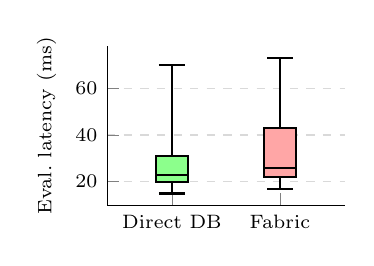
\begin{tikzpicture}
    \begin{axis}[panel, ylabel={Eval.\ latency (ms)},
      xmin=0.4, xmax=2.6, xtick={1,2}, xticklabels={Direct DB, Fabric},
      ymin=10, ymax=78, boxplot/draw direction=y,
      boxplot={draw position=\plotnum+1, box extend=0.3}]
    \addplot[boxplot prepared={median=23, upper quartile=31, lower quartile=20, upper whisker=70, lower whisker=15}, fill=green!45, draw=black] coordinates {};
    \addplot[boxplot prepared={median=26, upper quartile=43, lower quartile=22, upper whisker=73, lower whisker=17}, fill=red!35, draw=black] coordinates {};
    \end{axis}
    \end{tikzpicture}
    \caption{E4: ledger overhead}
    \end{subfigure}\hfill
    \begin{subfigure}[b]{0.32\textwidth}\centering
    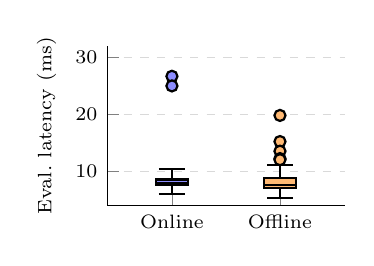
\begin{tikzpicture}
    \begin{axis}[panel, ylabel={Eval.\ latency (ms)},
      xmin=0.4, xmax=2.6, xtick={1,2}, xticklabels={Online, Offline},
      ymin=4, ymax=32, boxplot/draw direction=y,
      boxplot={draw position=\plotnum+1, box extend=0.3}]
    \addplot[boxplot prepared={median=7.8, upper quartile=8.5, lower quartile=7.5, upper whisker=10.4, lower whisker=6.0}, fill=blue!45, draw=black] coordinates {(1,26.7) (1,25.0)};
    \addplot[boxplot prepared={median=7.5, upper quartile=8.8, lower quartile=7.0, upper whisker=11.0, lower whisker=5.3}, fill=orange!55, draw=black] coordinates {(2,15.2) (2,13.5) (2,12.2) (2,12.0) (2,19.8)};
    \end{axis}
    \end{tikzpicture}
    \caption{E5: edge autonomy}
    \end{subfigure}
    \caption{Distribution plots for E1, E4, and E5. (a)~E1: median authorization latency for cloud PDP ($57.81$~ms, 50~ms WAN emulated) vs.\ edge PDP ($6.89$~ms); (b)~E4: evaluation latency boxplots for direct database write (median $23$~ms) vs.\ Hyperledger Fabric anchoring (median $26$~ms, overhead $+3$~ms); (c)~E5: edge PDP latency distribution under online and offline (WAN-severed) conditions, showing $100\%$ local availability with comparable latency.}
  \label{fig:s-e145}
\end{figure}

\begin{figure}[htbp]
\centering
\begin{subfigure}[b]{0.32\textwidth}\centering
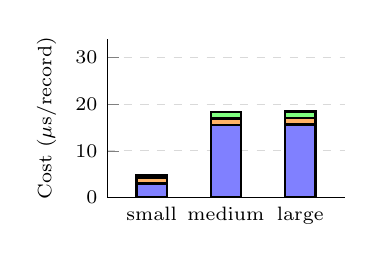
\begin{tikzpicture}
\begin{axis}[panel, ybar stacked, bar width=11pt, ylabel={Cost ($\mu$s/record)},
  xtick={1,2,3}, xticklabels={small, medium, large}, xmin=0.4, xmax=3.6, ymin=0, ymax=34]
\addplot[fill=blue!50] coordinates {(1,3.04)(2,15.61)(3,15.66)}; \label{plt:s:pseudo}
\addplot[fill=orange!60] coordinates {(1,1.16)(2,1.32)(3,1.33)}; \label{plt:s:gen}
\addplot[fill=green!50] coordinates {(1,0.54)(2,1.33)(3,1.45)}; \label{plt:s:redact}
\end{axis}
\end{tikzpicture}
\caption{E8: Minimizer per-stage cost}
\end{subfigure}\hfill
\begin{subfigure}[b]{0.32\textwidth}\centering
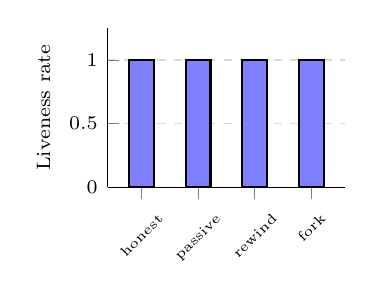
\begin{tikzpicture}
\begin{axis}[panel, ybar, bar width=9pt, ylabel={Liveness rate},
  xtick={1,2,3,4}, xticklabels={honest, passive, rewind, fork},
  x tick label style={font=\tiny, rotate=45}, xmin=0.4, xmax=4.6, ymin=0, ymax=1.25]
\addplot[fill=blue!50, draw=black] coordinates {(1,1.0)(2,1.0)(3,1.0)(4,1.0)};
\end{axis}
\end{tikzpicture}
\caption{E11: liveness ($0$ $\mathsf{INV}_{\mathrm{mono}}$ violations in 200 commits)}
\end{subfigure}\hfill
\begin{subfigure}[b]{0.32\textwidth}\centering
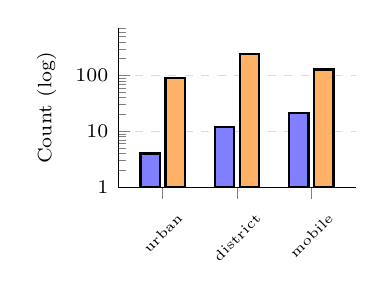
\begin{tikzpicture}
\begin{axis}[panel, ybar, bar width=7pt, ymode=log, log ticks with fixed point, ylabel={Count (log)},
  xtick={1,2,3}, xticklabels={urban, district, mobile},
  x tick label style={font=\tiny, rotate=45}, xmin=0.4, xmax=3.6, ymin=1, ymax=700]
\addplot[fill=blue!50, draw=black] coordinates {(1,4)(2,12)(3,21)}; \label{plt:s:part}
\addplot[fill=orange!60, draw=black] coordinates {(1,90)(2,240)(3,128)}; \label{plt:s:backlog}
\end{axis}
\end{tikzpicture}
\caption{E12: per-site partitions and backlog}
\end{subfigure}
\caption{Companion plots: (a) E8 Data Minimizer per-stage median cost (pseudonymize \ref{plt:s:pseudo}, generalize \ref{plt:s:gen}, redact \ref{plt:s:redact}); (b) E11 liveness under Byzantine behaviours; (c) E12 per-site partition count \ref{plt:s:part} and peak queue backlog \ref{plt:s:backlog} ($100\%$ availability at all sites).}
\label{fig:s-e81112}
\end{figure}

\section{E12 Per-Site Table and Real-Fabric Transcript}
\label{s:tables}

% \begin{table}[h]
% \centering
% \caption{E12 three-site partition/soak emulation, 720 simulated minutes, 29 cloud-side policy updates (seed 20260704).}
% \label{tab:s-soak}
% \footnotesize
% \setlength{\tabcolsep}{5pt}
% \begin{tabular}{lrrrrrrr}
% \toprule
% \textbf{Site} & \textbf{Requests} & \textbf{Avail.} & \textbf{Offline dec.} & \textbf{Stale dec.} & \textbf{Partitions} & \textbf{Max backlog} & \textbf{Max missed} \\
% \midrule
% Urban hospital  & 12{,}960 & 100\% & 270   & 36  & 4  & 90  & 1 \\
% District clinic & 8{,}640  & 100\% & 1{,}740 & 828 & 12 & 240 & 2 \\
% Mobile unit     & 5{,}760  & 100\% & 1{,}464 & 400 & 21 & 128 & 2 \\
% \midrule
% \textbf{Aggregate} & 27{,}360 & 100\% & 3{,}474 & 1{,}264 & 37 & 240 & 2 \\
% \bottomrule
% \end{tabular}
% \end{table}

\begin{table}[h]
\centering
\caption{E12 three-site partition/soak emulation, 720 simulated minutes, 29 cloud-side policy updates (seed 20260704).}
\label{tab:s-soak}
\footnotesize
\setlength{\tabcolsep}{4pt}
\begin{tabular}{lrrrrrrr}
\toprule
\textbf{Site} & \textbf{Requests} & \textbf{Avail.} & \shortstack[r]{\textbf{Offline}\\\textbf{dec.}} & \shortstack[r]{\textbf{Stale}\\\textbf{dec.}} & \textbf{Partitions} & \shortstack[r]{\textbf{Max}\\\textbf{backlog}} & \shortstack[r]{\textbf{Max}\\\textbf{missed}} \\
\midrule
Urban ward gwy. & 12{,}960 & 100\% & 270   & 36  & 4  & 90  & 1 \\
District clinic & 8{,}640  & 100\% & 1{,}740 & 828 & 12 & 240 & 2 \\
Mobile unit     & 5{,}760  & 100\% & 1{,}464 & 400 & 21 & 128 & 2 \\
\midrule
\textbf{Aggregate} & 27{,}360 & 100\% & 3{,}474 & 1{,}264 & 37 & 240 & 2 \\
\bottomrule
\end{tabular}
\end{table}

\noindent All $27{,}360$ decisions were logged to LogChain with zero loss after queue drains; mean reconciliation cost was $\approx 0.01$~ms per event in the in-process emulation. Stale decisions ($4.6\%$ of total) are decisions taken against a superseded but hash-verified policy version during a partition; all were reconciled by Phase~C.

\smallskip\noindent\textbf{Real-Fabric transcript summary.}
The official Hyperledger Fabric test network (two organizations, Raft ordering) was deployed with a JavaScript policy-hash chaincode on channel \texttt{acaaschan}: $8/8$ \texttt{invoke\_create} transactions succeeded with median $164$~ms and P95 $191$~ms; $8/8$ ledger reads returned within the retry window with median $137$~ms; final channel height was 16. This run is a feasibility check for the latency constants assumed in Eq.~(4) of the main paper, not a re-run of the mock-based E10/E11 sweeps.

\section{Reproduction Instructions}
\label{s:repro}

The artefact is available at \url{https://github.com/SonHaXuan/ACaaS} and was last executed with Python~3.12.3.

\begin{itemize}[leftmargin=*]
  \item \texttt{pytest -q} --- runs the full test suite (54 tests, including the 21-assertion G1--G5 conformance suite under \texttt{tests/security/}); completes in seconds.
  \item \texttt{python -m benchmarks.run\_all} --- regenerates every E6--E12 figure (PDF) and the underlying JSON result files under \texttt{results/}.
  \item \texttt{docker-compose up} --- brings up the full cloud--fog--edge stack on a single host for interactive exploration.
  \item \texttt{results/manifest.sha256} --- checksums of the result bundle used in the paper.
\end{itemize}

\end{document}
